\documentclass[letterpaper]{article}
\usepackage{amsmath}
\usepackage{tikz}
\usepackage{epigraph}
\usepackage{lipsum}

\renewcommand\epigraphflush{flushright}
\renewcommand\epigraphsize{\normalsize}
\setlength\epigraphwidth{0.7\textwidth}

\definecolor{titlepagecolor}{cmyk}{1,.60,0,.40}

\DeclareFixedFont{\titlefont}{T1}{ppl}{b}{it}{0.5in}

\makeatletter
\def\printauthor{%
    {\large \@author}}
\makeatother
\author{%
    Nico Taljaard \\
    10153285 \vspace{20pt} \\
    Gerhard Smit \\
    12282945 \vspace{20pt} \\
    Martin Schoeman \\
    10651994 \\
}

% The following code is borrowed from: http://tex.stackexchange.com/a/86310/10898

\newcommand\titlepagedecoration{%
	\begin{tikzpicture}[remember picture,overlay,shorten >= -10pt]
	
		\coordinate (aux1) at ([yshift=-15pt]current page.north east);
		\coordinate (aux2) at ([yshift=-410pt]current page.north east);
		\coordinate (aux3) at ([xshift=-4.5cm]current page.north east);
		\coordinate (aux4) at ([yshift=-150pt]current page.north east);
		
		\begin{scope}[titlepagecolor!40,line width=12pt,rounded corners=12pt]
			\draw
			  (aux1) -- coordinate (a)
			  ++(225:5) --
			  ++(-45:5.1) coordinate (b);
			\draw[shorten <= -10pt]
			  (aux3) --
			  (a) --
			  (aux1);
			\draw[opacity=0.6,titlepagecolor,shorten <= -10pt]
			  (b) --
			  ++(225:2.2) --
			  ++(-45:2.2);
		\end{scope}
			\draw[titlepagecolor,line width=8pt,rounded corners=8pt,shorten <= -10pt]
			  (aux4) --
			  ++(225:0.8) --
			  ++(-45:0.8);
		\begin{scope}[titlepagecolor!70,line width=6pt,rounded corners=8pt]
			\draw[shorten <= -10pt]
			  (aux2) --
			  ++(225:3) coordinate[pos=0.45] (c) --
			  ++(-45:3.1);
			\draw
			  (aux2) --
			  (c) --
			  ++(135:2.5) --
			  ++(45:2.5) --
			  ++(-45:2.5) coordinate[pos=0.3] (d);   
			\draw 
			  (d) -- +(45:1);
		\end{scope}
	\end{tikzpicture}
}

\begin{document}

\begin{titlepage}

\noindent
\titlefont Laminin \par
\epigraph{ Team portfolio used in tenders applycations for the project presented in Cos301 Software Engineering by the University of Pretoria. This document intoduces all the team members to have a beter understanding of who we are and why our skills are suitable for this project.}%
{\textit{ 2014 }\\ \textsc{ }}
\null\vfill
\vspace*{1cm}
\noindent
\hfill
\begin{minipage}{0.35\linewidth}
    \begin{flushright}
        \printauthor
    \end{flushright}
\end{minipage}
%
\begin{minipage}{0.02\linewidth}
    \rule{1pt}{125pt}
\end{minipage}
\titlepagedecoration
\end{titlepage}

% % % % % % % % % % % % % % %
% 							%
%	Remainder of document	%
% 							%
% % % % % % % % % % % % % % % 

	\newpage
	
	\begin{flushleft}
		\begin{figure}[ht!]
			\fbox{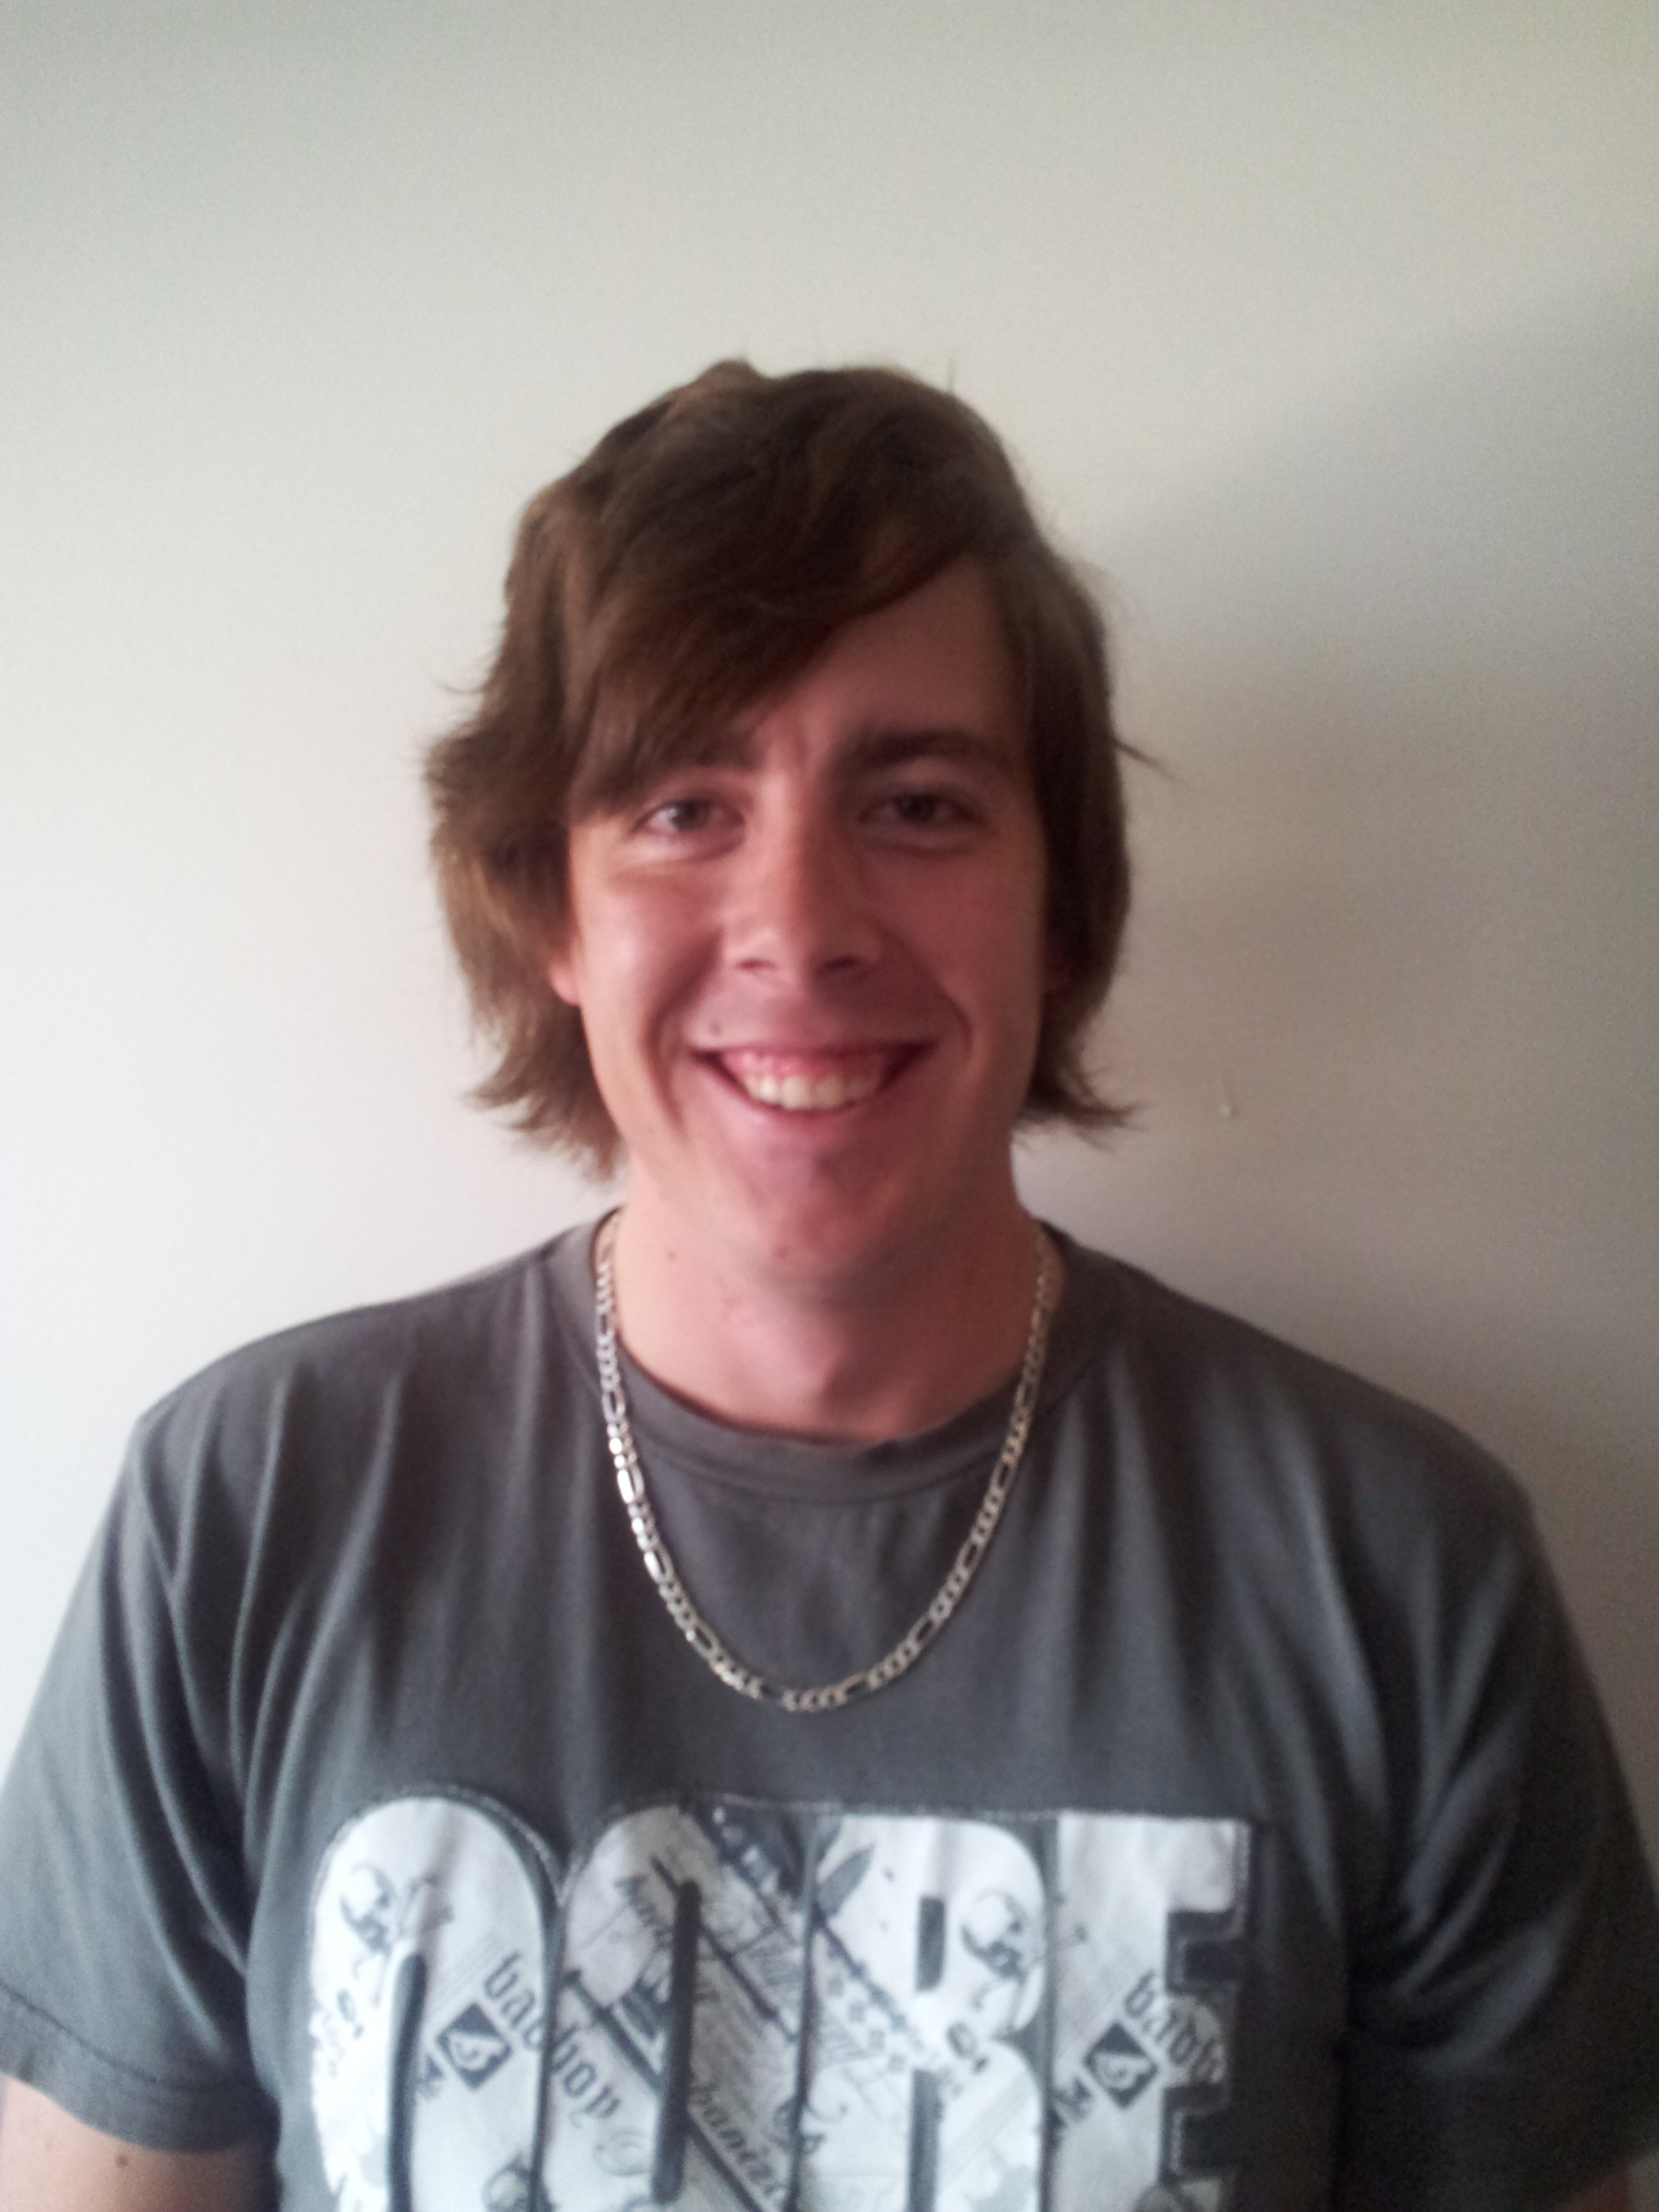
\includegraphics[width=2in, height=2in]{./Fotos/NicoTaljaard.jpg}}
		\end{figure}
	\end{flushleft}
			
	\vspace{0.1in}
	
	\vspace*{0.2in}
	\begin{minipage}{0.26\linewidth}
		Name 			\\
		Surname			\\
		Contact Info 	\\
						\\
		Field of Study	\\
						\\
		Skills			\\
						\\
						\\
						\\
						\\
		Work Experience	\\
						\\
						\\
		Additional Info	\\
						\\
						\\
		Interests		\\
						\\
	\end{minipage}
 	%
	\begin{minipage}{0.02\linewidth}
		\rule{1pt}{250pt}
	\end{minipage}
	%
	\begin{minipage}{0.85\linewidth}
		Nico \\
		Taljaard \\
		0827323108 \\
		taljaard.nj@gmail.com \\
		BSc Computer Science \\
		
		Programming languages: Java, C++, C, OpenGL 4.0, EBNF \\
		Databasing: PostgreSQL, MySQL, DB4O, BaseX, SQLserver \\
		Design and Implementation: HTML, CSS, PHP, XML \\ 
		Graphic Design: Maya, 3dsMax \\
		
		2014 - University of Pretoria Teaching Assistant \\
		2014 - Software Developer At Willa Krause \\
		
		Team leader and worker. Good time management, people skills and productive worker. \\
		
		I enjoy playing games, watching series, movies and reading fiction books. \\
	\end{minipage}
		
	\titlepagedecoration



	\newpage
		
	\begin{flushleft}
		\begin{figure}[ht!]
			\fbox{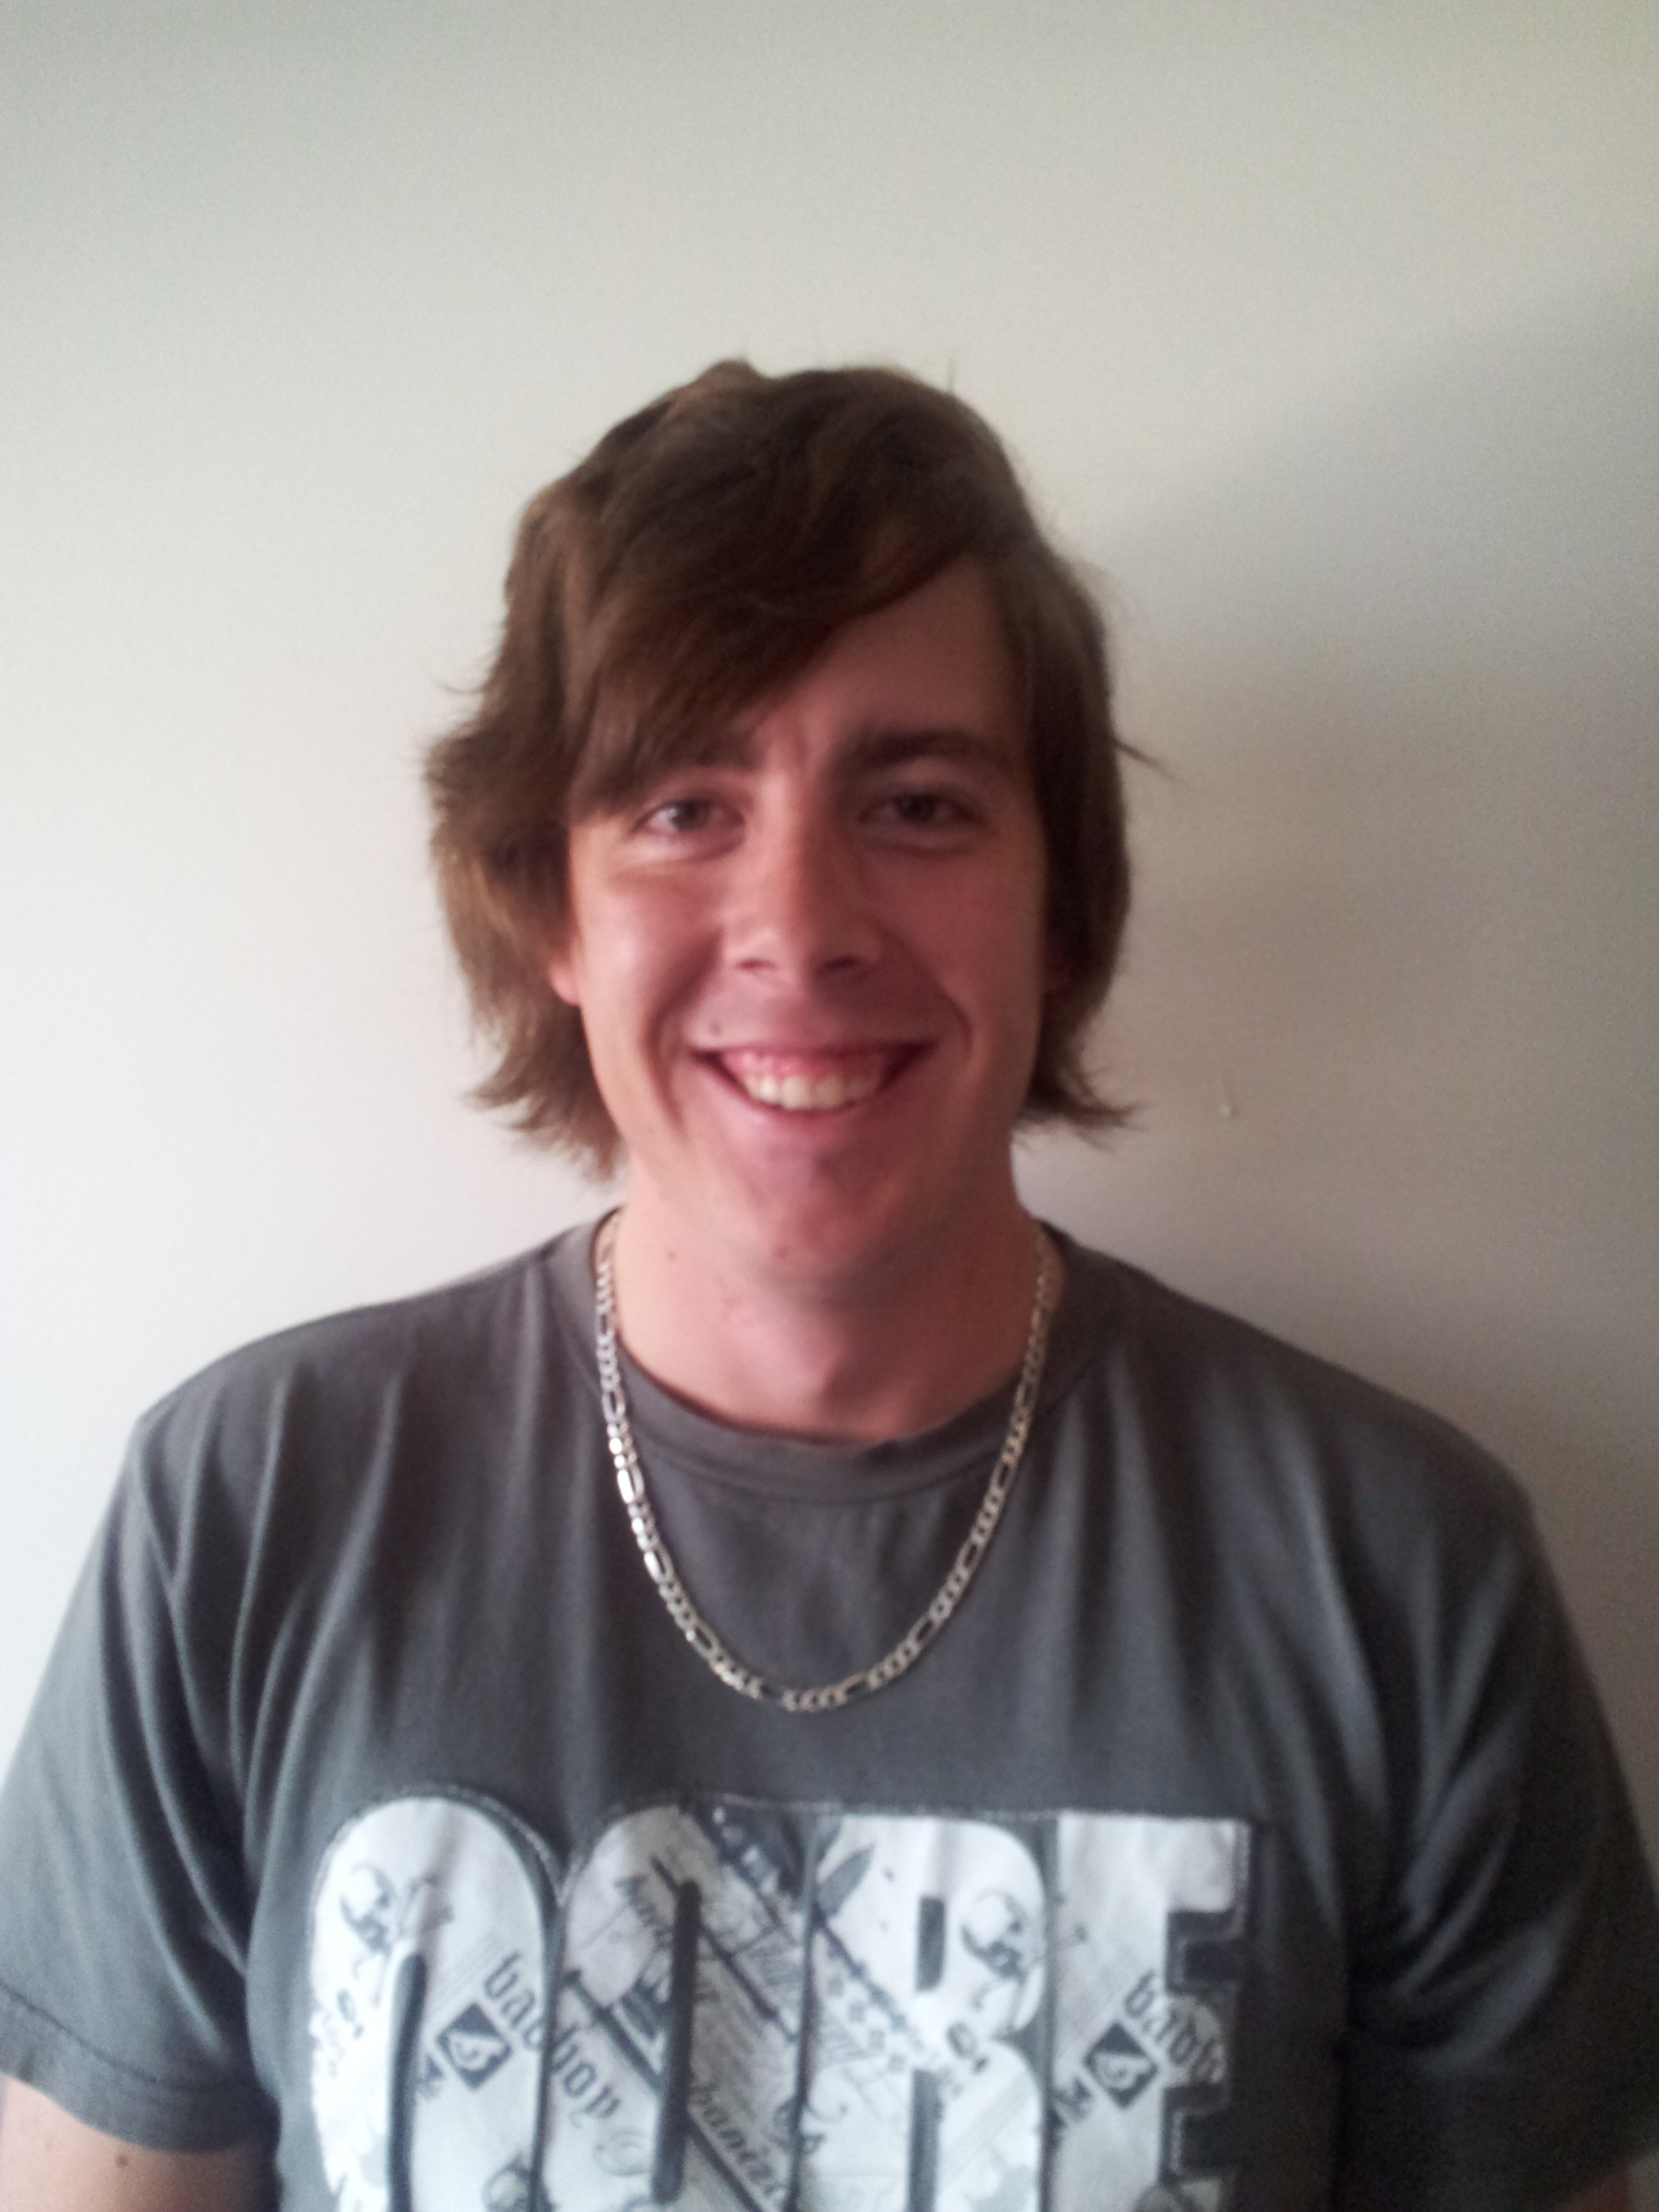
\includegraphics[width=2in, height=2in]{./Fotos/NicoTaljaard.jpg}}
		\end{figure}
	\end{flushleft}
			
	\vspace{0.1in}
	
	\vspace*{0.2in}
	\begin{minipage}{0.26\linewidth}
			Name 			\\
			Surname			\\
			Contact Info 	\\
							\\
			Field of Study	\\
							\\
			Skills			\\
							\\
							\\
							\\
			Work Experience	\\
							\\
							\\
			Additional Info	\\
							\\
							\\
							\\
			Interests		\\
							\\
							\\
	\end{minipage}
 	%
	\begin{minipage}{0.02\linewidth}
		\rule{1pt}{250pt}
	\end{minipage}
	%
	\begin{minipage}{0.85\linewidth}
		Gerhard \\
		Smit \\
		0788936745 \\
		gsmit16@gmail.com \\
		BSc Computer Science \\
						
		Programming languages: Java, C++, OpenGL 4.0 \\
		Databasing: MySQL, SQLserver \\
		Design and Implementation: HTML, CSS, PHP, XML \\ 
		
		2012 - 2014 - Purple pepper Maths Tutor \\
		2013 - 2014 - University of Pretoria Teaching Assistant \\

		Hard worker, good follower as well as the capability to lead, excellent people skills. Never backs down from a challenge, always willing to help. \\
						
		I love playing PC games, I enjoy watching epic films and horrors. Exploring nature and hanging out with friends. \\
		Love eating out and trying out new things. \\

	\end{minipage}
	
	\titlepagedecoration



	\newpage
		
	\begin{flushleft}
		\begin{figure}[ht!]
			\fbox{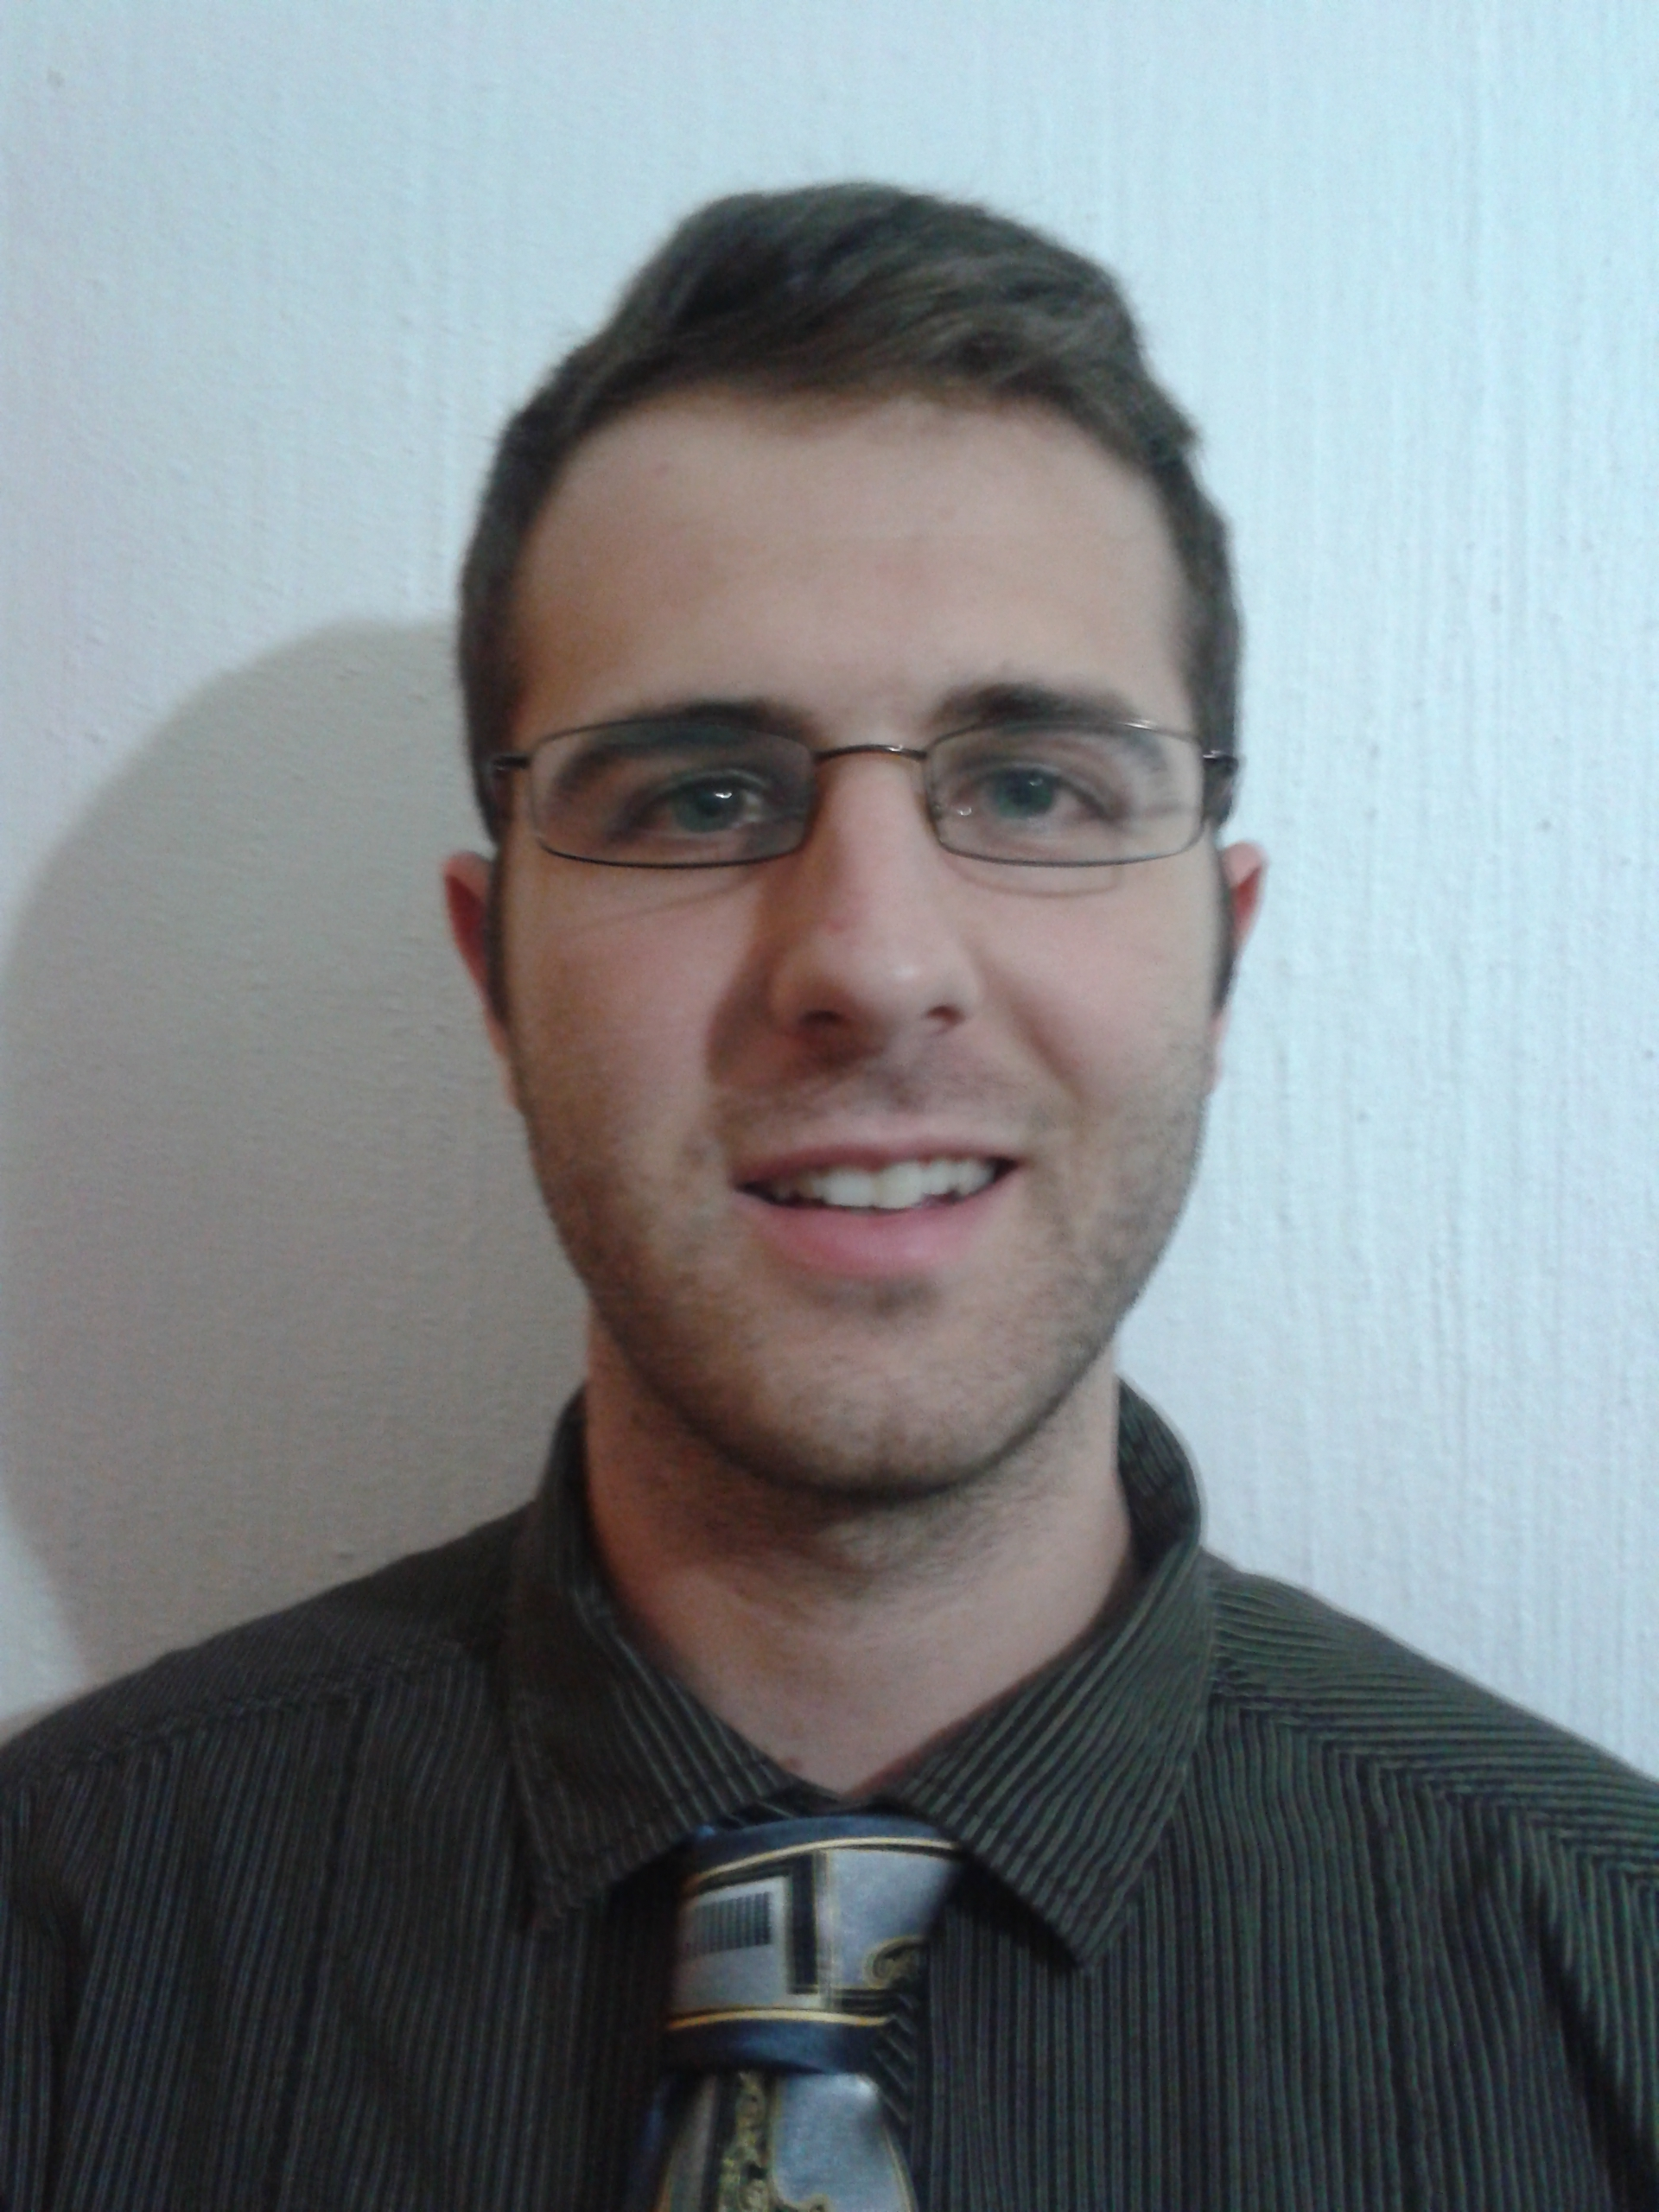
\includegraphics[width=2in, height=2in]{./Fotos/Martin.jpg}}
		\end{figure}
	\end{flushleft}
			
	\vspace{0.1in}
	
	\vspace*{0.2in}
	\begin{minipage}{0.26\linewidth}
		Name 			\\
		Surname			\\
		Contact Info 	\\
						\\
		Field of Study	\\
						\\
		Skills			\\
						\\
						\\
						\\
		Work Experience	\\
						\\
						\\
						\\
						\\
		Additional Info	\\
						\\
						\\
		Interests		\\
						\\
	\end{minipage}
 	%
	\begin{minipage}{0.02\linewidth}
		\rule{1pt}{250pt}
	\end{minipage}
	%
	\begin{minipage}{0.85\linewidth}
		Martin \\
		Schoeman \\
		072 997 2698 \\
		mjschoeman69@gmail.com \\
		BSc IT Software Development \\
		
		Programming languages: C Sharp, C++, Delphi, Java,  \\
		Databasing: PostgreSQL, MySQL, DB4O, BaseX, SQLserver \\
		Design and Implementation: HTML, CSS, PHP, XML \\ 
		
		2011 - Business Genetics Programmer \\
		2012 - University of Pretoria Mentor  \\
		2013 - University of Pretoria Mentor  \\
		2014 - University of Pretoria Mentor  \\
		
		Enjoy programming and solving programming problems.\\
		Also trying the help others when they are struggling.\\  
		
		I have interest in rugby, bikes and computer games, like league of legends. \\
	\end{minipage}
		
	\titlepagedecoration


\end{document}